%
% LaTeX report template 
%

% This is a comment: in LaTeX everything that in a line comes
% after a "%" symbol is treated as comment

\documentclass[11pt, a4paper]{article}
\usepackage{graphicx}
\usepackage{amsmath}
\usepackage{listings}
\usepackage{url}

\title{Assignment 4: Fourier Approximations} % Title

\author{Nithin Babu [EE18B021]} % Author name

\date{\today} % Date for the report
\begin{document}	
		
\maketitle % Insert the title, author and date
\section*{Abstract}
%Create new section;it is autonumbered
The goal of this assignment is the following.
\begin{itemize}
\item To fit two functions $e^{x}$ and $cos(cos(x))$ using the Fourier series.
\item To use least squares fitting to simplify the process of calculating Fourier series.
\item To plot graphs to understand the above
\end{itemize}


\section{The functions $e^{x}$ and $cos(cos(x))$}
The following python snippet is used to declare the functions $e^{x}$ and $cos(cos(x))$. The x values are also declared from -2$\pi$ to 4$\pi$.

\begin{verbatim}
def expo(x):
    return exp(x)

def coscos(x):
    return cos(cos(x))
	
x = linspace(-2*pi,4*pi,1200)
y_exp = expo(x)
y_coscos = coscos(x)
\end{verbatim}

The following code is used to plot the graphs of $e^{x}$ and $cos(cos(x))$.
\begin{verbatim}
figure(1)
semilogy(x,y_exp,label='True')
title("Figure 1")
xlabel(r'$x\rightarrow$',size=15)
ylabel(r'$e^x\rightarrow$',size=15)
grid(True)
legend()
\end{verbatim}
The plots of $e^{x}$ and $cos(cos(x))$ are as shown below:
   \begin{figure}[!tbh]
   	\centering
   	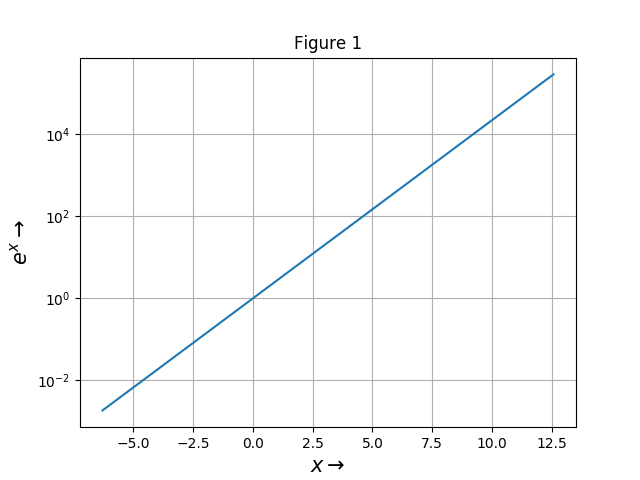
\includegraphics[scale=0.6]{Figure_1.png}   
   	\caption{Data plot}
   	\label{fig:sample}
   \end{figure} 
   
   \begin{figure}[!tbh]
   	\centering
   	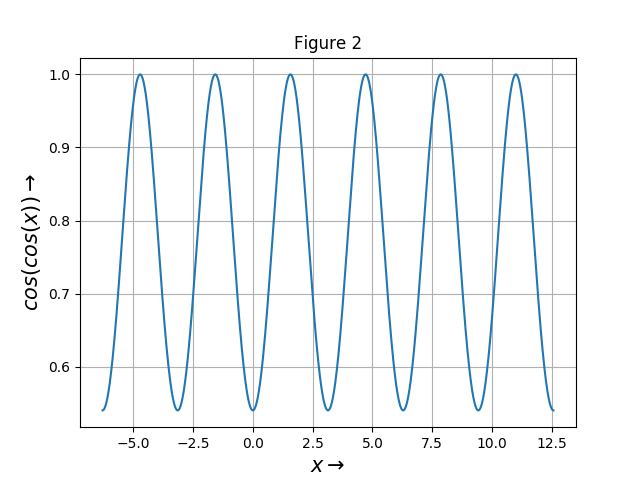
\includegraphics[scale=0.6]{Figure_2.png}   
   	\caption{Data plot}
   	\label{fig:sample}
   \end{figure} 
   As it is evident from the plots, $e^{x}$ is aperiodic whereas $cos(cos(x))$ is periodic. The functions generated by the fourier series should be a periodic extension of the actual functions. The plots showing the periodic extensions of $e^{x}$ and $cos(cos(x))$ are as shown below:
   \begin{figure}[!tbh]
   	\centering
   	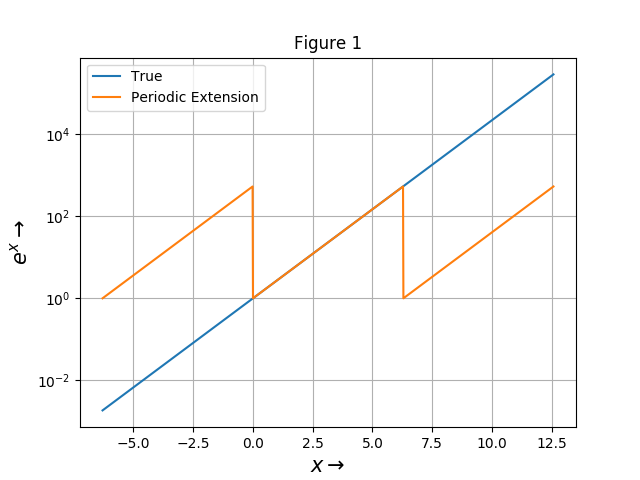
\includegraphics[scale=0.6]{Figure_1p.png}   
   	\caption{Data plot}
   	\label{fig:sample}
   \end{figure} 
   
   \begin{figure}[!tbh]
   	\centering
   	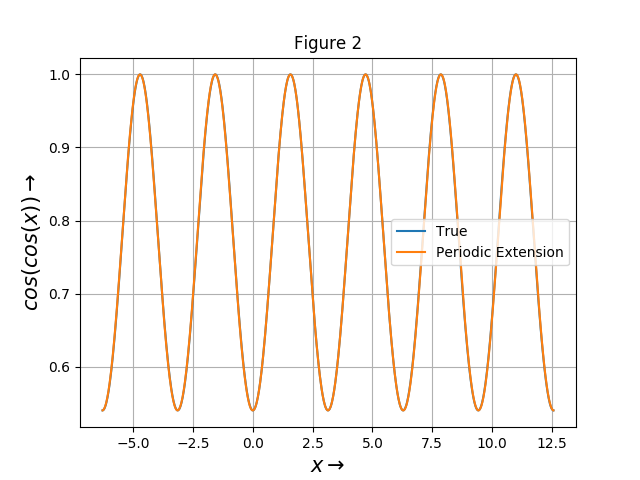
\includegraphics[scale=0.6]{Figure_2p.png}   
   	\caption{Data plot}
   	\label{fig:sample}
   \end{figure} 

\section{The Fourier coefficients}
The fourier series used to approximate a function is as follows:
\begin{equation}
    a_{0} + \sum\limits_{n=1}^{\infty} {{a_{n}\cos(nx_{i})+b_{n}\sin(nx_{i})}} \approx f(x_{i}) 
    \end{equation}
    	The equations used here to find the Fourier coefficients are as follows:
    \begin{equation}
         a_{0} = \frac{1}{2\pi}\int\limits_{0}^{2\pi} f(x)dx 
    \end{equation}
    \begin{equation}
         a_{n} = \frac{1}{\pi}\int\limits_{0}^{2\pi} f(x)\cos(nx)dx 
    \end{equation}
    \begin{equation}
         b_{n} = \frac{1}{\pi}\int\limits_{0}^{2\pi} f(x)\sin(nx)dx 
    \end{equation}

Hence, in python we will use the \textit{quad()} function to perform an intergration function. First we'll have to create functions which contains the variable $k$ also. The python code snippet for declaring the functions with an additional variable $k$ is as follows:
\begin{verbatim}
def u_exp(x,k):
	return expo(x)*cos(k*x)

def u_coscos(x,k):
	return coscos(x)*cos(k*x)	

def v_exp(x,k):
	return expo(x)*sin(k*x)

def v_coscos(x,k):
	return coscos(x)*sin(k*x)	

\end{verbatim}
The python code snippet for finding the fourier coefficients is as follows:
\begin{verbatim}
for k in range(26):
	
    a_exp = integrate.quad(u_exp,0,2*pi,args=(k))[0]/pi
    b_exp = integrate.quad(v_exp,0,2*pi,args=(k))[0]/pi
    a_coscos = integrate.quad(u_coscos,0,2*pi,args=(k))[0]/pi
    b_coscos = integrate.quad(v_coscos,0,2*pi,args=(k))[0]/pi

    if k==0:
        sum_exp += a_exp/2
        sum_coscos += a_coscos/2
        c_exp[p][0]  = a_exp/2
        c_coscos[p][0] = a_coscos/2 
        p = p + 1

    else:
        sum_exp += a_exp*cos(k*x) + b_exp*sin(k*x)	
        sum_coscos += a_coscos*cos(k*x) + b_coscos*sin(k*x)	
        c_exp[p][0] = a_exp
        c_coscos[p][0] = a_coscos
        c_exp[p+1][0] = b_exp
        c_coscos[p+1][0] = b_coscos
        p = p + 2
\end{verbatim}
   
\section{The plots of Fourier coefficients}
The semilog and log plots of the Fourier coefficients of  $e^{x}$ and $cos(cos(x))$ is as shown:
	\begin{figure}[!tbh]
   	\centering
   	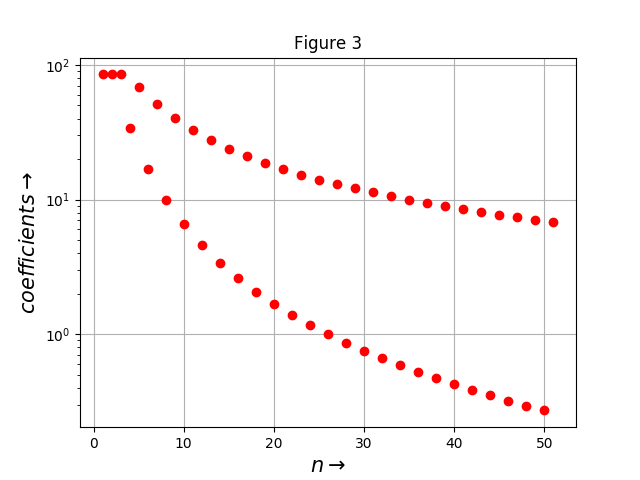
\includegraphics[scale=0.6]{Figure_3.png}   
   	\caption{Semilog plot of the fourier coefficients of $e^{x}$}
   	\label{fig:sample}
   \end{figure} 

	\begin{figure}[!tbh]
   	\centering
   	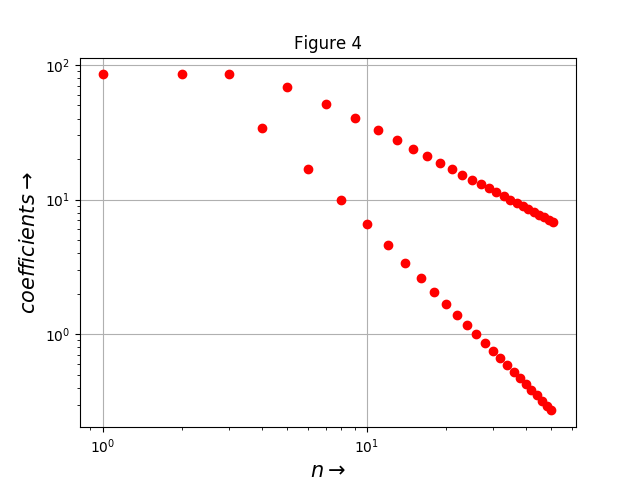
\includegraphics[scale=0.6]{Figure_4.png}   
   	\caption{Log plot of the fourier coefficients of $e^{x}$}
   	\label{fig:sample}
   \end{figure} 
   
	\begin{figure}[!tbh]
   	\centering
   	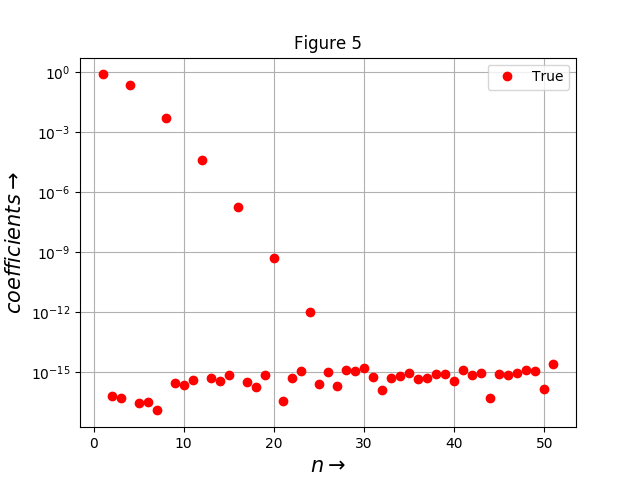
\includegraphics[scale=0.6]{Figure_5.png}   
   	\caption{Semilog plot of the fourier coefficients of $cos(cos(x))$}
   	\label{fig:sample}
   \end{figure} 

	\begin{figure}[!tbh]
   	\centering
   	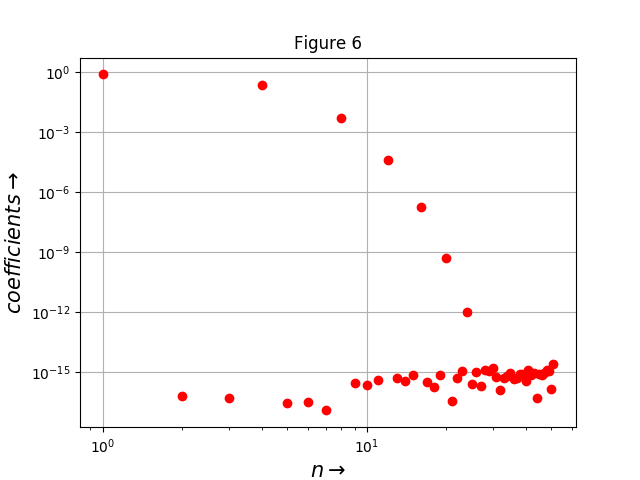
\includegraphics[scale=0.6]{Figure_6.png}   
   	\caption{Log plot of the fourier coefficients of $cos(cos(x))$}
   	\label{fig:sample}
   \end{figure} 

a. As it is evident from the plots, $b_n$ is nearly zero for $cos(cos(x))$. This is because $cos(cos(x))$ is an even function, hence in the fourier series expansion, all the $b_n$ terms should be zero for the series to be an even function.\\\\
b. The magnitude of the coefficients would represent how much of certain frequencies happen to be in the output. $cos(cos(t))$ does not have very many frequencies of harmonics, so it dies out quickly. However, since the periodic extension of $e^{t}$ is discontinuous. To represent this discontinuity as a sum of continuous sinusoids, we would need high frequency components, hence coefficients do not decay as quickly.\\\\
c. The loglog plot is linear for $e^{t}$ since Fourier coefficients of $e^{t}$ decay with $1/n$ or $1/n^{2}$. The semilog plot seems linear in the $cos(cos(t))$ case as its fourier coefficients decay exponentially with n.

\section{The Least Squares Approach}
For the least squares approach, we'll have to create matrices and then use \textit{lstsq()} function inorder to get the most approximate values of the fourier coefficients.\\
The python code snippet to create the matrices and to get the least squared value of the coefficients is as follows:
\begin{verbatim}	
xl=linspace(0,2*pi,401)
xl=xl[:-1] 

B_exp = expo(xl)
B_coscos = coscos(xl) 

A = zeros((400,51))
A[:,0] = 1
for k in range(1,26):
    A[:,2*k-1] = cos(k*xl)
    A[:,2*k] = sin(k*xl)

cl_exp = lstsq(A,B_exp,rcond=None)[0]
cl_coscos = lstsq(A,B_coscos,rcond=None)[0]
\end{verbatim}
The plots in order to show the differences between the actual and predicted values of the fourier coefficients are shown below

	\begin{figure}[!tbh]
   	\centering
   	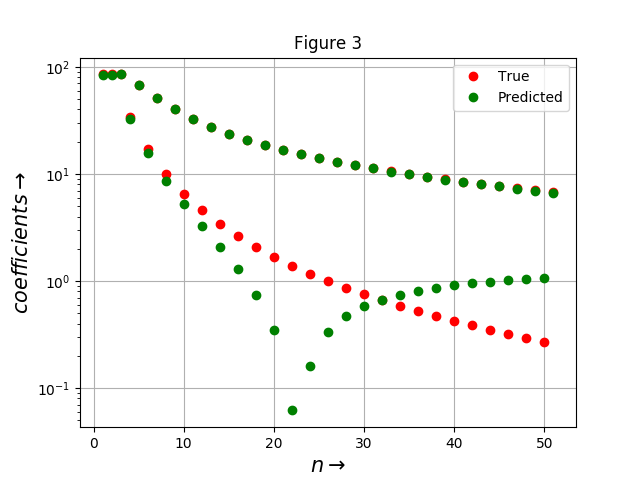
\includegraphics[scale=0.6]{Figure_7.png}   
   	\caption{Semilog plots for $e^{x}$}
   	\label{fig:sample}
   \end{figure} 
   
   \begin{figure}[!tbh]
   	\centering
   	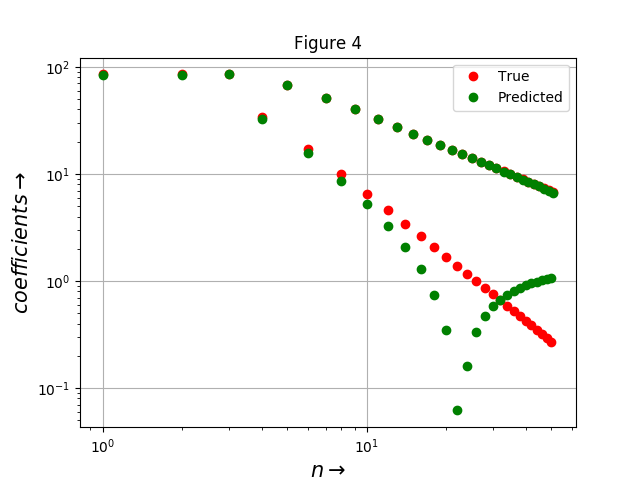
\includegraphics[scale=0.6]{Figure_8.png}   
   	\caption{Log plots for $e^{x}$}
   	\label{fig:sample}
   \end{figure} 
   
   \begin{figure}[!tbh]
   	\centering
   	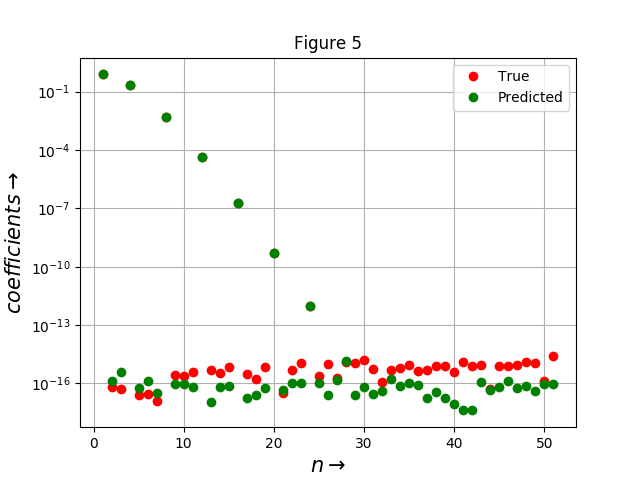
\includegraphics[scale=0.6]{Figure_9.png}   
   	\caption{Semilog plots for $cos(cos(x))$}
   	\label{fig:sample}
   \end{figure} 
   
   \begin{figure}[!tbh]
   	\centering
   	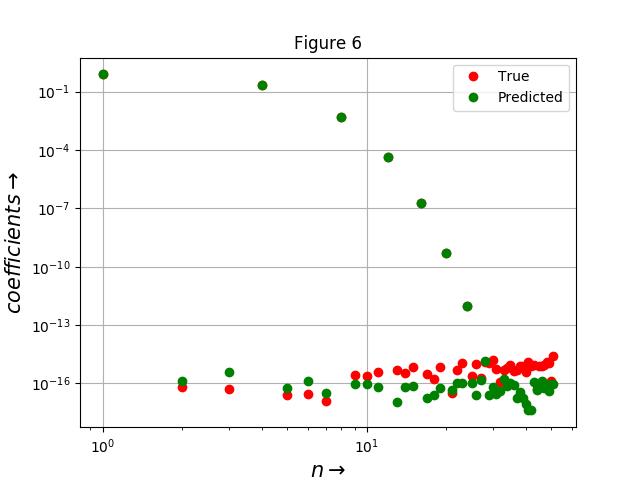
\includegraphics[scale=0.6]{Figure_10.png}   
   	\caption{Log plots for $cos(cos(x))$}
   	\label{fig:sample}
   \end{figure} 
     
\section{Deviation from Actual Values} 
The least squares approach is still an approximate method and will definitely have a slight deviation from the actual value.\\
The following python code snippet is used to calculate the deviation:
\begin{verbatim}	
diff_exp = abs(cl_exp - c_exp)
diff_coscos = abs(cl_coscos - c_coscos)

dev_exp = diff_exp.max()
dev_coscos = diff_coscos.max()
\end{verbatim}
The deviation in the case of $e^{x}$ is 170.1304798\\
The deviation in the case of $cos(cos(x))$ is 0.9950046\\\\
There is very good agreement in values in the case of $cos(cos(x))$ but a significant amount of difference in the case of $e^{t}$. The reason for this is that the periodic extension of the exponential function is discontinuous, and hence would require a lot more samples to accurately determine its Fourier coefficients. If we increased the number of samples to $10^{6}$, the maximum deviation would reduce, but not vanish.
The effect of this lack of samples is felt more near the discontinuity of the signal.


\section{Estimated Functions}
Using the predicted values of the fourier coefficients, we can calculate the functional values for both $e^{x}$ and $cos(cos(x))$. \\
The plots showing both the actual and predicted functional values are as shown below:

 	\begin{figure}[!tbh]
   	\centering
   	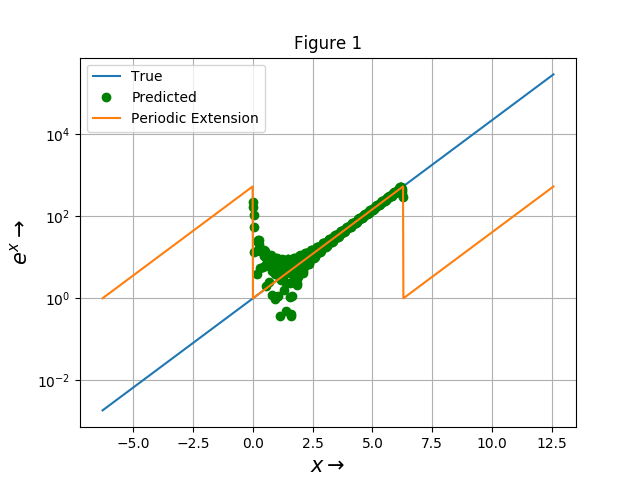
\includegraphics[scale=0.6]{Figure_1a.png}   
   	\caption{Actual and predicted values for $e^{x}$}
   	\label{fig:sample}
   \end{figure} 
   
   \begin{figure}[!tbh]
   	\centering
   	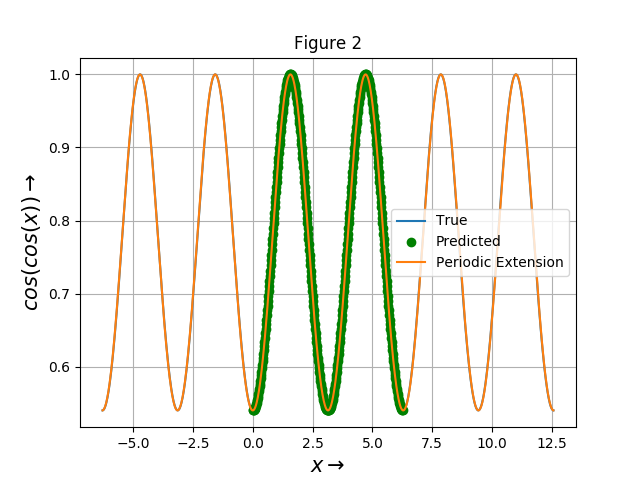
\includegraphics[scale=0.6]{Figure_2a.png}   
   	\caption{Actual and predicted values for $cos(cos(x))$}
   	\label{fig:sample}
   \end{figure} 
   The $cos(cos(t))$ vs t graph, agrees almost perfectly, beyond the scope of the precision of the least squares fitter.
The Fourier approximation of $e^{t}$ does not agree very well to the ideal case near the discontinuity. The cause for this is the Gibbs Phenomenon, which can be described as below.
The partial sums of the Fourier series will have large oscillations near the discontinuity of the function. These oscillations do not die out as n increases, but approaches a finite limit.
This is one of the causes of ringing artifacts in signal processing, and is very undesirable.
Plotting the output on a linear graph would make this ringing much more apparent.
	
\section*{Conclusions}
\begin{itemize}
\item We saw two different ways to calculate the Fourier series of a periodic signal.
\item We saw how least squares fitting can be used to simplify the process of calculating the Fourier Series.
\item We observed Gibbs phenomenon at the discontinuity in the Fourier approximation of $e^{t}$.
\end{itemize}

\end{document}